\documentclass[12pt]{article}
\usepackage[margin=2.5cm]{geometry}
\usepackage{enumerate}
\usepackage{amsfonts}
\usepackage{amsmath}
\usepackage{fancyhdr}
\usepackage{amsmath}
\usepackage{amssymb}
\usepackage{amsthm}
\usepackage{mdframed}
\usepackage{graphicx}
\usepackage{subcaption}
\usepackage{adjustbox}
\usepackage{listings}
\usepackage{xcolor}
\usepackage{booktabs}
\usepackage[utf]{kotex}
\usepackage{hyperref}

\definecolor{codegreen}{rgb}{0,0.6,0}
\definecolor{codegray}{rgb}{0.5,0.5,0.5}
\definecolor{codepurple}{rgb}{0.58,0,0.82}
\definecolor{backcolour}{rgb}{0.95,0.95,0.92}

\lstdefinestyle{mystyle}{
    backgroundcolor=\color{backcolour},
    commentstyle=\color{codegreen},
    keywordstyle=\color{magenta},
    numberstyle=\tiny\color{codegray},
    stringstyle=\color{codepurple},
    basicstyle=\ttfamily\footnotesize,
    breakatwhitespace=false,
    breaklines=true,
    captionpos=b,
    keepspaces=true,
    numbers=left,
    numbersep=5pt,
    showspaces=false,
    showstringspaces=false,
    showtabs=false,
    tabsize=1
}

\lstset{style=mystyle}

\pagestyle{fancy}
\renewcommand{\headrulewidth}{0.4pt}
\lhead{CSC 373}
\rhead{Worksheet 2 Solution}

\begin{document}
\title{CSC373 Worksheet 2 Solution}
\maketitle

\bigskip

\begin{enumerate}[1.]
    \item

    \begin{center}
    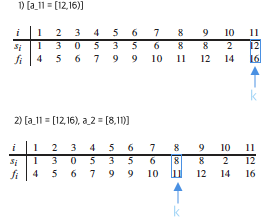
\includegraphics[width=\linewidth]{images/worksheet_2_solution_3.png}
    \end{center}

    \bigskip

    This approach is a greedy algorithm because algorithm

    \begin{enumerate}[1)]
        \item Has the greedy choice: selecting the last activity to start that is compatible
        with all previously selected activites

        \item Has the greedy choice that is always part of optimal solution:

        \bigskip

        \underline{\textbf{Claim:}}

        \bigskip

        Consider any nonempty subproblem $S_k$. Let $a_m$ be an activity in $S_k$
        with the last activity to start that is compatible with all previously selected
        activities. Then $a_m$ is included in some maximum-size subset of mutually
        compatible activities of $S_k$

        \begin{proof}
        Let $A_k$ be a maximum-size subset of mutually compatible activities in $S_k$,
        and let $a_j$ be the activity in $A_k$ with the last activity to start that is
        compatible with all previously selected activities.

        \bigskip

        If $a_j = a_m$, we are done, since we have shown that $a_m$ is the maximum-size
        subset of mutually compatible activities of $S_k$.

        \bigskip

        If $a_j \neq a_m$, let the set $A'_k = A_k = \{a_j\} \cup \{a_m\}$ be
        $A_k$ but subtituting $a_m$ for $a_j$. The activities in $A'_k$ are disjoint,
        which follow because the activities in $A_k$ are disjoint, $a_j$ is the
        first activity in $A_k$ to finish, and $s_j \leq s_m$.

        \bigskip

        Since $\lvert A'_k \rvert = \lvert A_k \rvert$, we conclude that $A'_k$
        is a maximum-size subset of mutually compatible activities of $S_k$, and it includes $a_m$.
        \end{proof}
    \end{enumerate}

    \bigskip

    \underline{\textbf{Notes:}}

    \bigskip

    \begin{itemize}
        \item Greedy Algorithm

        \begin{itemize}
            \item Always makes the choice that looks best at the moment

            \begin{itemize}
                \item Locally optimal solution leads to globally optimal solution
            \end{itemize}

        \end{itemize}

        \item Activity-selection Problem (Greedy algorithm using dynamic programming)

        \begin{itemize}
            \item Goal: Selecting maximum size set of mutually compatible activities

            \bigskip

            \underline{\textbf{Example:}}

            \bigskip

            \begin{tabular}{c|ccccccccccc}
                $i$ & 1 & 2 & 3 & 4 & 5 & 6 & 7 & 8 & 9 & 10 & 11\\
                \hline
                $s_i$ & 1 & 3 & 0 & 5 & 3 & 5 & 6 & 8 & 8 & 2 & 12\\
                $f_i$ & 4 & 5 & 6 & 7 & 9 & 9 & 10 & 11 & 12 & 14 & 16
            \end{tabular}

            \bigskip

            \item Suppose a set exists $S = \{a_1 = [s_1, f_1), a_2 = [s_2, f_2), ..., a_n = [s_n, f_n)\}$

            \begin{itemize}
                \item $a_i$ represents an $i^{th}$ activity
                \item $s_i$ represents starting time
                \item $f_i$ represents finishing time
                \item $0 \leq s_i < f_i < \infty$
                \item $a_1, ..., a_n$ sorted in monotonically increasing order of finish time

                \bigskip

                \quad i.e.

                \bigskip

                \quad $f_1 \leq f_2 \leq f_3 \leq ... \leq f_{n-1} \leq f_n$

                \bigskip

                \item $a_i$ and $a_j$ are \textbf{compatible}, if intervals $[s_i, f_i)$ and $[s_j, f_j)$
                don't overlap

                \bigskip

                \quad i.e

                \bigskip

                \quad $s_i \geq f_j$ and $s_j \geq f_i$

                \bigskip

            \end{itemize}

            \item Steps

            \begin{enumerate}[1.]
                \item Think about dynamic programming solution

                \begin{itemize}
                    \item Construct optimal solution using two subproblems

                    \begin{mdframed}

                    \textbf{$S_{ij}$:} activities that start after activity $a_i$ finishes and before
                    activity $a_j$ starts

                    \bigskip

                    i.e.

                    \bigskip

                    $S_{19} = \{a_4 = [5,7), a_6 = [5, 9), a_7 = [6, 10)\}$

                    \bigskip

                    \textbf{$A_{ij}$:} maximum set of mutually compatible activities in $S_{ij}$ (including $a_k$)

                    \begin{itemize}
                        \item $A_{ik} = A_{ij} \cap S_{ik}$
                        \item $A_{kj} = A_{ij} \cap S_{kj}$
                        \item $A_{ij} = A_{ik} \cup \{a_k\} \cup A{kj}$
                        \item So, $\lvert A_{ij} \rvert  = \lvert A_{ik} \rvert + \lvert A_{kj} \rvert + 1$
                    \end{itemize}

                    \end{mdframed}

                    \item Verify that optimal solution $A_{ij}$ must include optimal solution to the two subproblems
                    for  $S_{kj}$

                    \begin{mdframed}
                        Let $A'_{kj}$ be another mutually compatible activities in $S_{kj}$ where $\lvert A'_{kj} \rvert > \lvert A_{kj} \rvert$.

                        \bigskip

                        Then we could use $A'_{kj}$ in a solution to subproblem of $S_{ij}$

                        \bigskip

                        Then we have $\lvert A_{ik} \rvert + \lvert A'_{kj} \rvert + 1 > \lvert A_{jk} \rvert + \lvert A_{kj} \rvert + 1 = \lvert A_{ij} \rvert$ mutually compatible activites

                        \bigskip

                        This contradicts assumption that $A_{ij}$ is an optimal solution
                    \end{mdframed}

                    \item Verify that optimal solution $A_{ij}$ must include optimal solution to the two subproblems
                    for $S_{ik}$

                    \begin{mdframed}
                    The same applies for activities in $S_{ik}$
                    \end{mdframed}
                \end{itemize}

                \item Observe that only one choice - greedy choice, and that when we make the greedy choice, only one subproblem remains

                \begin{itemize}
                    \item Steps

                    \begin{enumerate}[1.]
                        \item Make a greedy choice
                        \begin{itemize}
                            \item Choose an activity that makes the most resource possible (intuition)
                            \item Choose an acitivty that finishes the earliest (intuition)
                        \end{itemize}
                        \item Solve a subproblem: Find activities that start after $a_1$ finishes
                        \item Verify that making greedy choices always arrive at optimal solution
                    \end{enumerate}
                \end{itemize}

                \bigskip

                \begin{mdframed}

                \underline{\textbf{Theorem 16.1 (Page 418):}}

                \bigskip

                Consider any non-empty subproble $S_k$, and let $a_m$ be an activity in $S_k$
                with the earliest finish time. Then $a_m$ is included in some maximum-size subset of
                mutually compatible activities of $S_k$

                \end{mdframed}
                \item Develop recursive greedy solution

                \begin{center}
                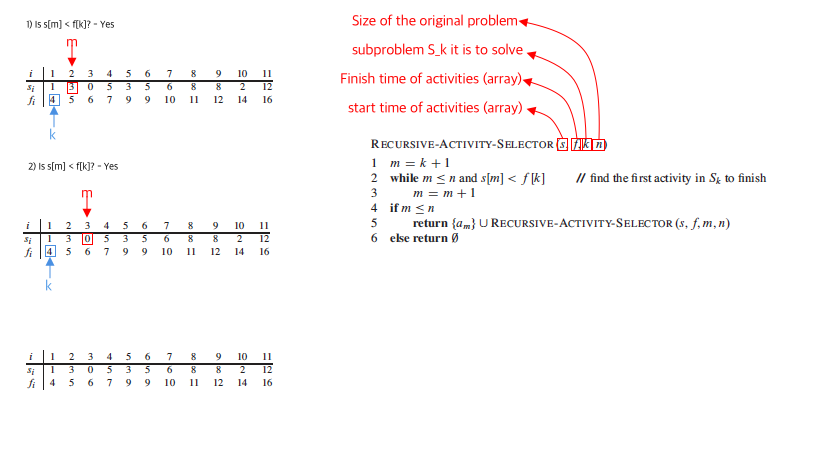
\includegraphics[width=\linewidth]{images/worksheet_2_solution_1.png}
                \end{center}


                \item Convert the recursive algorithm into iterative one

                \begin{center}
                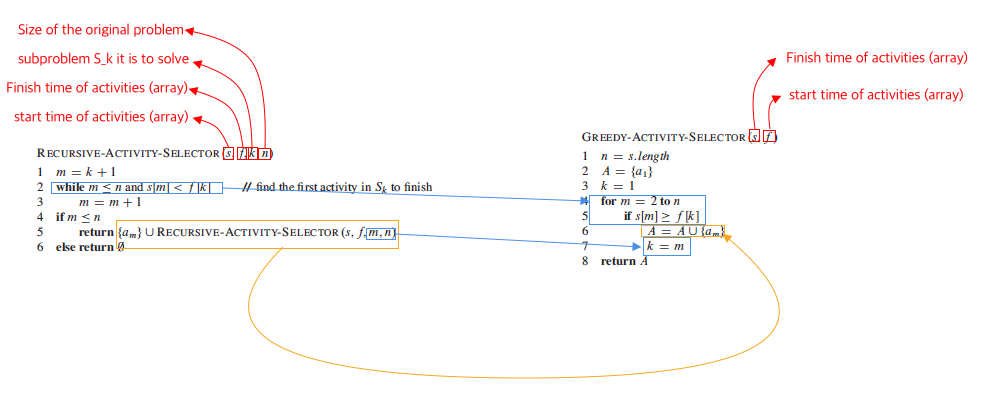
\includegraphics[width=\linewidth]{images/worksheet_2_solution_2.png}
                \end{center}
            \end{enumerate}
        \end{itemize}
    \end{itemize}

    \item

    \begin{itemize}
        \item Greedy Choice

        \begin{itemize}
            \item Choose $x_i$ that is greater than the current maximum as the upper bound
            of unit length closed interval
            \item Choose $x_i$ that is smaller than the current minimum as the lower bound of unit length
            closed interval
        \end{itemize}

        \bigskip

        \underline{\textbf{Example:}}

        \bigskip

        $\{0,1,2,3,4,5\}$ $\to$ $[0,5]$

        \bigskip

        $\{0,-1,3,5,2\}$ $\to$ $[-1,5]$

        \item Optimal Substructure

        \bigskip

        Let $I$ be the following instance of the problem: Let $n$ be the number of items,
        and let $x_i$ be the $i^{th}$ point in the set.

        \bigskip

        Let $A = [x_{\text{min}}, x_{\text{max}}]$ be the solution. The greedy algorithm works by assigning $x_{\text{min}} = min(x_{\text{min}}, x_n)$ and
        $x_{\text{max}} = max(x_{\text{max}}, x_n)$, and then continuing by solving the subproblem

        \begin{align}
            I' = (n - 1, \{x_1,..., x_{n-1}\})
        \end{align}

        until $n = 0$.

        \bigskip

        We need to show that the strategy gives optimal solution.

    \end{itemize}

    \bigskip

    \begin{mdframed}
        \underline{\textbf{Correct Solution:}}

        \color{red}
        \begin{enumerate}[1)]
            \item Consider the left-most interval.
            \item Set the left most point $x$ in the set as its value (since we know it must contain the leftmost point)
            \item For any point that is within the unit distance of the point $x$ (i.e. $[x, x+1]$), remove the points
            since they are covered
            \item Move to the next closest point not covered by the unit interval of $x$, and repeat until all points in the set are covered.
            \item Since each step has a clearly optimal choice for where to put the leftmost interval, the final solution is optimal
        \end{enumerate}

        \color{black}

        \bigskip

    \end{mdframed}

    \underline{\textbf{Notes:}}

    \bigskip

    \begin{itemize}
        \item I stopped because it's taking too much time.
        \item I struggled on this problem.

        \begin{itemize}
            \item I had trouble understanding the meaning of unit interval
            \item I felt there is missing knowledge regarding optimal substructure
            \item I felt tunnel visioned to provide one interval that covers all
        \end{itemize}

        \item I had difficulty arguing why the algorith is correct

        \begin{itemize}
            \item i.e. How can i generate a claim?
        \end{itemize}

        \item Unit length

        \begin{itemize}
            \item $[1,25, 2.25]$ includes all $x_i$ such that $1.25 \leq x_i \leq 2.25$.
        \end{itemize}
        \item Greedy-choice property and optimal substructure to problem are the two key ingredients
        \item Summary of Steps for Greedy Algorithm

        \begin{enumerate}[1.]
            \item Determine the optimal structure of the problem
            \item Develop a recursive solution.
            \item Show that if we make the greedy choice, then only one subproblem remains
            \item Prove that it is always safe to make the greedy choice
            \item Develop a reursive algorithm that implements the greedy strategy
            \item Convert the recursive algorithm to an iterative algorithm
        \end{enumerate}

        % \item Steps to Designing Greedy Algorithm

        % \begin{enumerate}[1.]
        %     \item Cast the optimization problem as one in which we make a choice and are left
        %     with one subproblem to solve
        %     \item Prove that there is always an optimal solution to the original problem that makes
        %     the greedy choice, so that the greedy choice is always safe
        %     \item Demonstrate optimal substructure by showing that having made the greedy
        %     choice, what remains is a subproblem with the property that if we combine an
        %     optional solution to the subproblem with the greedy choice we have made,
        %     we arrive at an optimal solution to the original problem
        % \end{enumerate}

        \item Criteria for Greedy Algorithm
        \begin{enumerate}[1.]
            \item Greedy-choice property

            \begin{itemize}
                \item Exists if we can assemble a globally optimal solution by making a
                locally optimal (greedy) choices
            \end{itemize}

            \item Optimal Substructure

            \begin{itemize}
                \item Exists if an optimal solution to the problem contains within it
                optimal solutions to subproblems.
            \end{itemize}
        \end{enumerate}

        \item Greedy vs Dynamic Programming

        \begin{itemize}
            \item 0-1 Knapsack Problem

            \begin{center}
            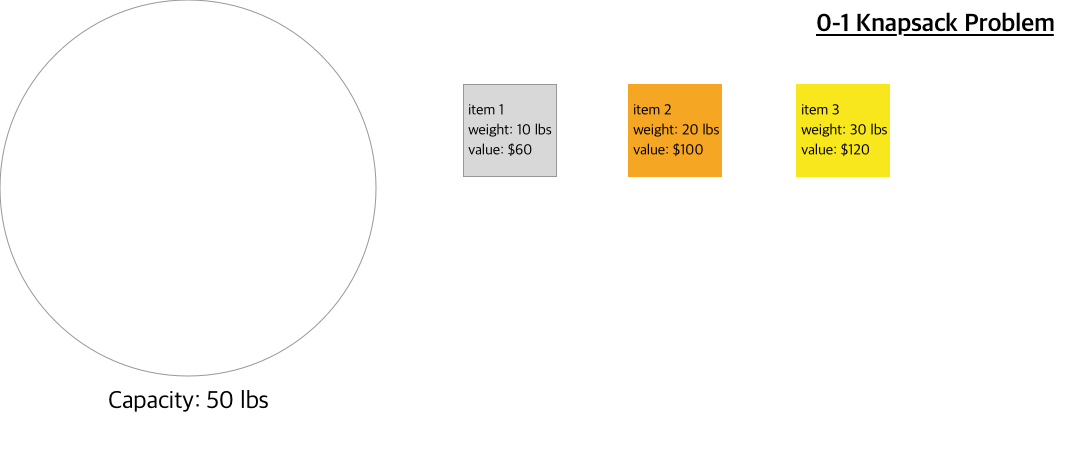
\includegraphics[width=\linewidth]{images/worksheet_2_solution_4.png}
            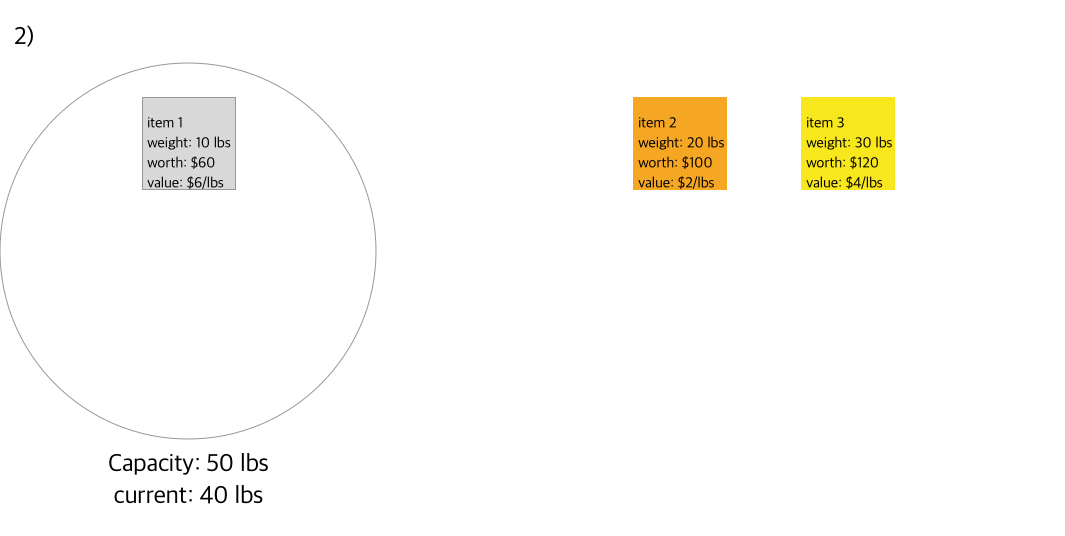
\includegraphics[width=\linewidth]{images/worksheet_2_solution_5.png}
            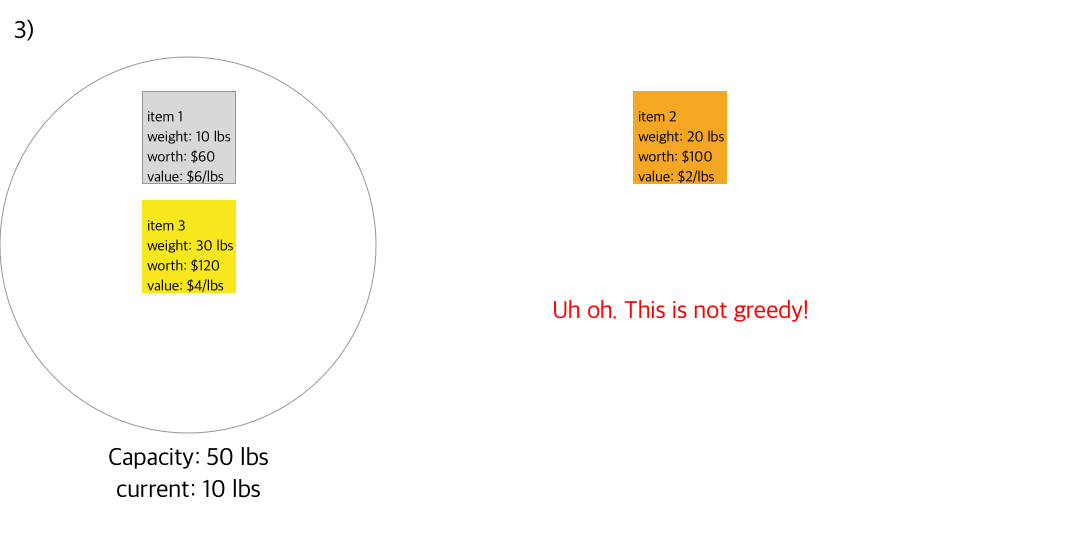
\includegraphics[width=\linewidth]{images/worksheet_2_solution_6.png}
            \end{center}

            \item Fractional Knapsack Problem

            \begin{center}
            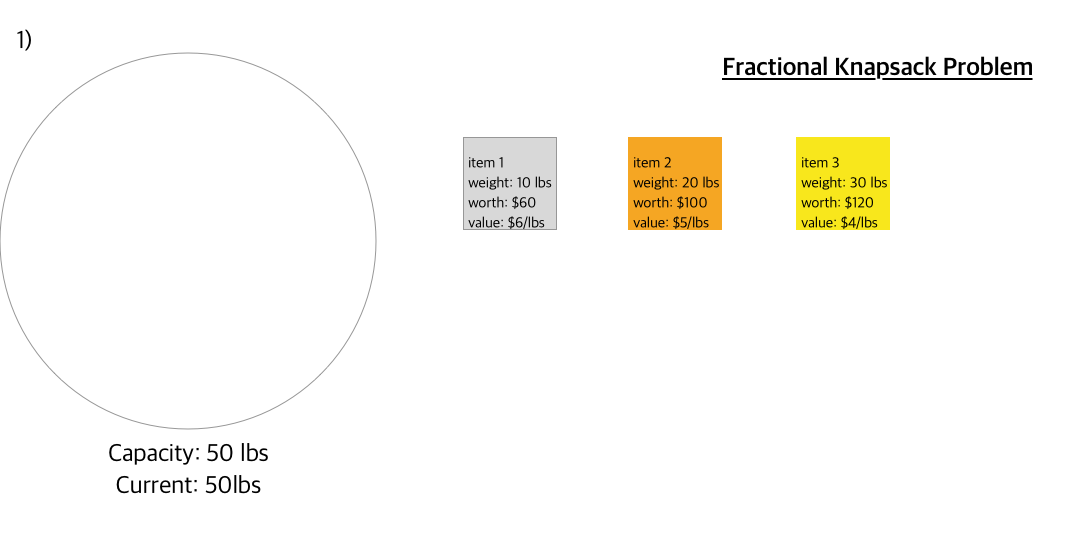
\includegraphics[width=\linewidth]{images/worksheet_2_solution_7.png}
            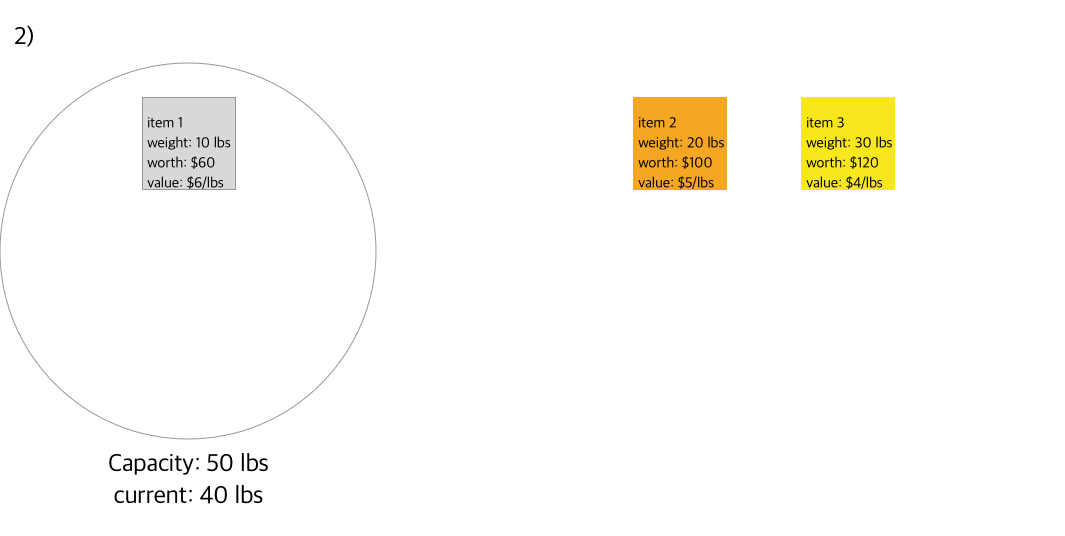
\includegraphics[width=\linewidth]{images/worksheet_2_solution_8.png}
            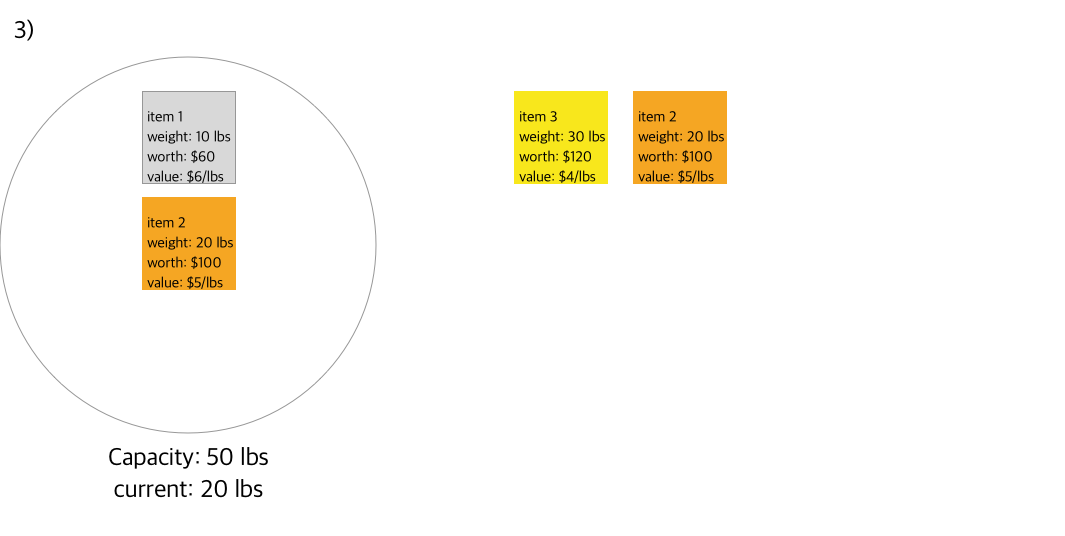
\includegraphics[width=\linewidth]{images/worksheet_2_solution_9.png}
            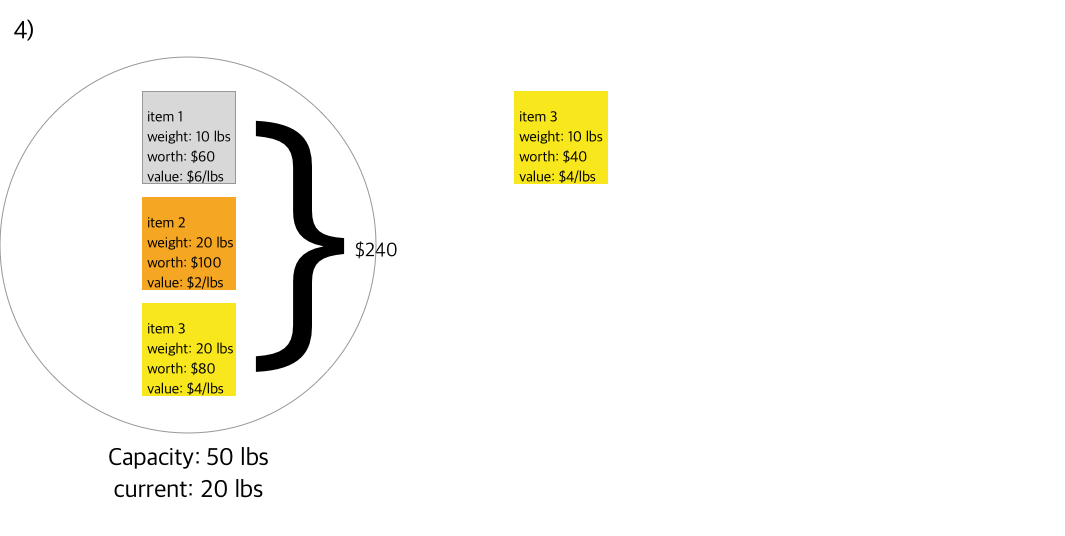
\includegraphics[width=\linewidth]{images/worksheet_2_solution_10.png}
            \end{center}
        \end{itemize}
    \end{itemize}

    \item
    \setcounter{equation}{0}

    \begin{proof}

    Let $T$ be a binary tree corresponding to an optimal prefix code and suppose
    that $T$ is not full. Let node $n$ have a single child $x$. Let $T'$ be the
    tree obtained by removing $n$ and replacing it by $x$. Let $m$ be leaf node
    which is descendent of $x$. Then we have:


    \begin{mdframed}
    \underline{\textbf{My work:}}

    \begin{align}
    B(T') &\leq \sum\limits_{c \in C \setminus \{m\}} c.freq \cdot d_T(c) + m.freq \cdot d_{T'}(m)\\
    &= \sum\limits_{c \in C \setminus \{m\}} c.freq \cdot d_T(c) + m.freq \cdot (d_T(m) - 1)\\
    &< \sum\limits_{c \in C \setminus \{m\}} c.freq \cdot d_T(c) + m.freq \cdot d_T(m)\\
    &= \sum\limits_{c \in C} c.freq \cdot d_T(c)\\
    &= B(T)
    \end{align}

    \end{mdframed}

    which contradicts the fact that $T$ was optimal. Therefore every binary tree
    corresponding to an optimal prefix code is full

    \end{proof}

    \underline{\textbf{Notes:}}

    \bigskip

    \begin{itemize}
        \item Optimal Substructure

        \begin{itemize}
            \item A problem is said to have optimal substructure if an optimal solution
            can be constructed from optimal solutions of its subproblems.
        \end{itemize}

        \item Huffman Codes

        \begin{itemize}
            \item Is an algorithm that uses greedy algorithm for lossless (without loss of data) data compression
            \item Has two types of codewords

            \begin{center}
            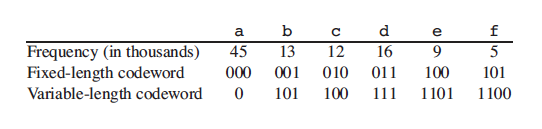
\includegraphics[width=\linewidth]{images/worksheet_2_solution_11.png}
            \end{center}

            \begin{itemize}
                \item Fixed Length Code

                \begin{itemize}
                    \item has codeword with the same length
                \end{itemize}

                \item Variable Length
                \begin{itemize}
                    \item has codeword that may be of different lengths
                \end{itemize}
            \end{itemize}
            \item Constructs optimal prefix codes

            \begin{itemize}
                \item Means no codeword is a prefix of some other codewords

                \bigskip

                e.g.

                The following is not prefix codes

                \bigskip

                a - 110

                b - 1101

                \bigskip

                e.g.

                The following is prefix codes

                \bigskip

                a - 110

                b - 111

                \bigskip
            \end{itemize}
        \end{itemize}

        \item Realized that I should learn with the solution. Otherwise, it will take too much time.
        \item Learned that the author used another but very similar tree $T'$ to show the cost of
        bits in $T$ is not minimum, which is the condition of prefix codes.
        \item Learned that the solution feels very similar to the proof of optimal
        substructure on page 416.
        \item Learned that the tree $T$ and $T'$ looks as follows:

        \begin{center}
        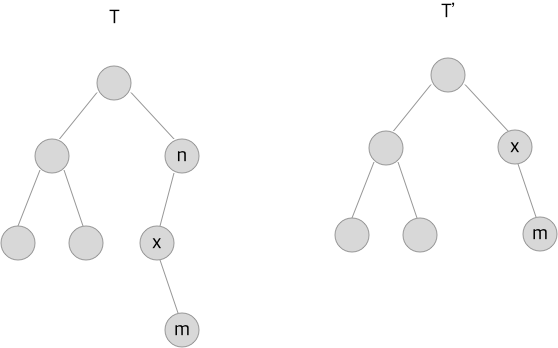
\includegraphics[width=\linewidth]{images/worksheet_2_solution_12.png}
        \end{center}

    \end{itemize}

    \item

    \bigskip

    \underline{\textbf{Solution:}}

    \begin{itemize}
        \item Finding optimal Huffman code

        \begin{center}
        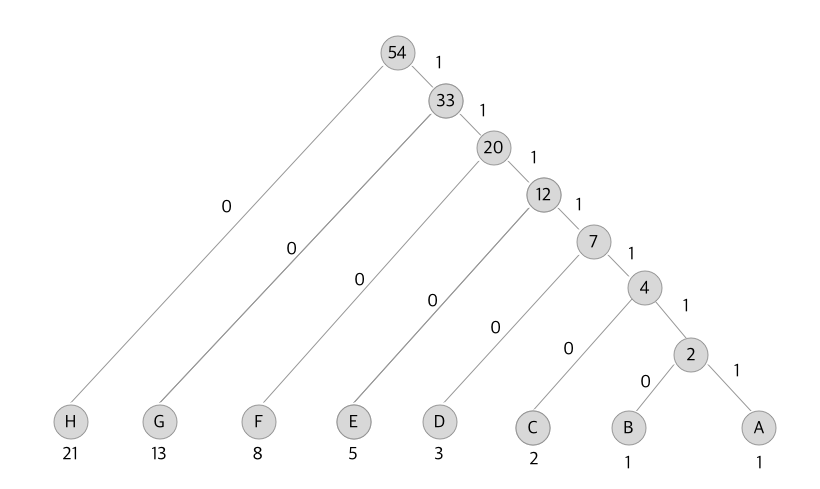
\includegraphics[width=\linewidth]{images/worksheet_2_solution_19.png}
        \end{center}

        \item Generalizing answer to find the optimal code when the frequencies are
        first $n$ fibonacci numbers

        \begin{center}
        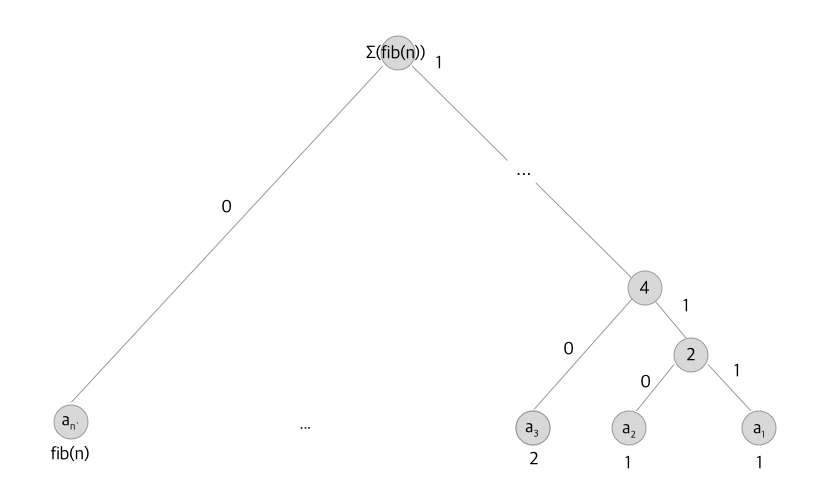
\includegraphics[width=\linewidth]{images/worksheet_2_solution_20.png}
        \end{center}

    \end{itemize}

    \underline{\textbf{Notes}}

    \bigskip

    \begin{itemize}
        \item Constructing Huffman Code

        \bigskip

        \underline{\textbf{Example:}}

        \bigskip

        \begin{tabular}{|c|c|c|c|c|c|c|c|}
            \hline
            char & A & E & I & S & T & P & $\backslash$ n\\
            Freq & 10 & 15 & 12 & 3 & 4& 13 & 1\\
            \hline
        \end{tabular}

        \begin{enumerate}[1.]
            \item Take the 2 chars with the lowest frequency

            \begin{center}
            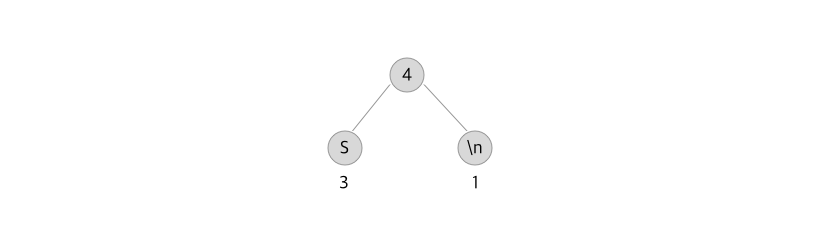
\includegraphics[width=\linewidth]{images/worksheet_2_solution_13.png}
            \end{center}

            \item Make a 2 leaf node tree from them

            \begin{center}
            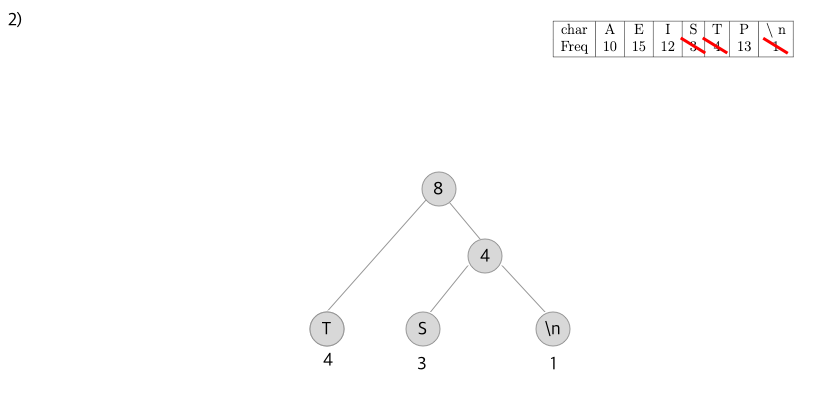
\includegraphics[width=\linewidth]{images/worksheet_2_solution_14.png}
            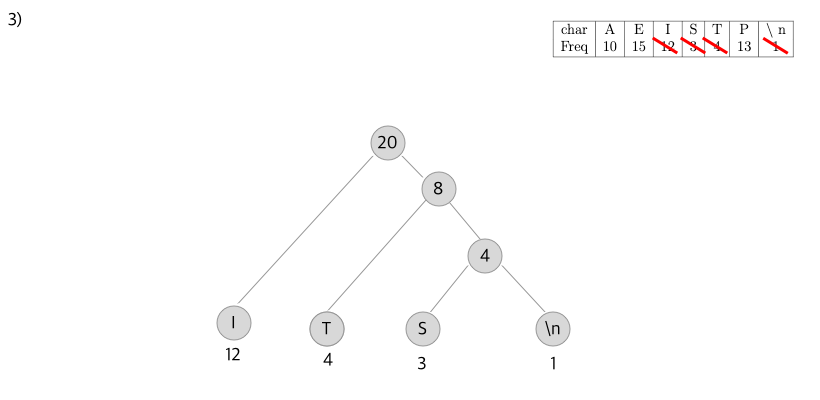
\includegraphics[width=\linewidth]{images/worksheet_2_solution_15.png}
            \end{center}

            \item If the node has summed value that is higher than any other values in the table,
            then repeat 1 and 2 in another tree

            \begin{center}
            
\includegraphics[width=\linewidth]{images/worksheet_2_solution_16.png}
            \end{center}

            \item Attach an additional node to the subtree with the smallest value


            \begin{center}
            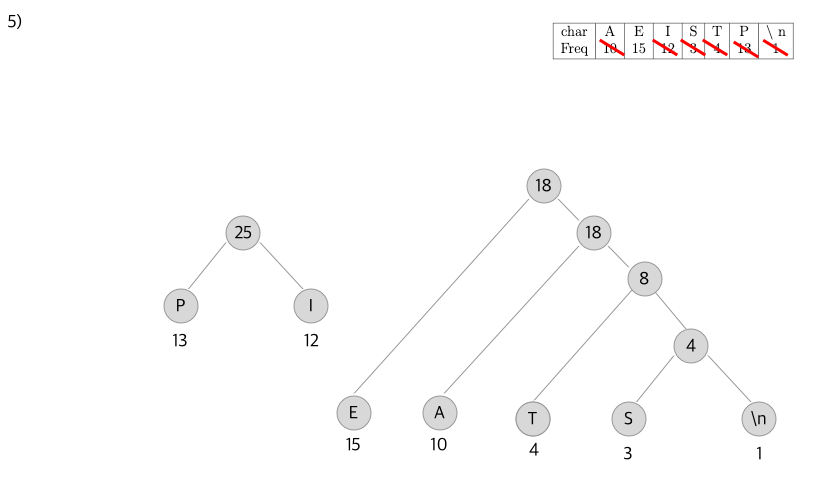
\includegraphics[width=\linewidth]{images/worksheet_2_solution_17.png}
            \end{center}

            \item Repeat step 4 above until done

            \begin{center}
            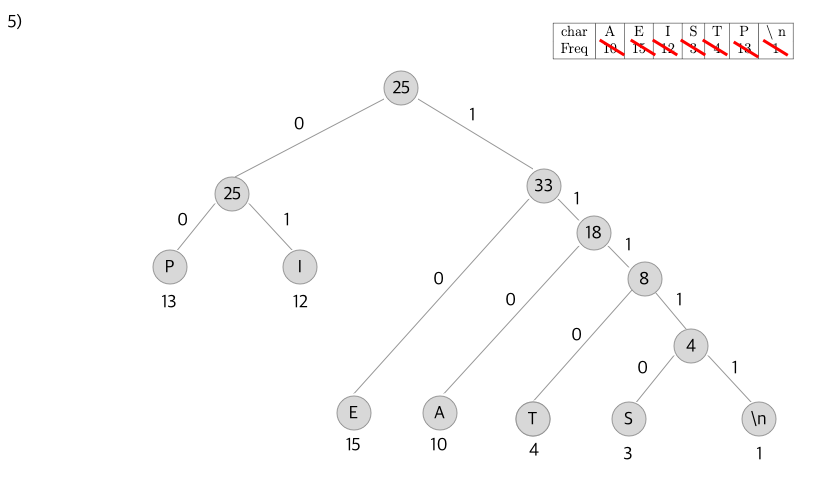
\includegraphics[width=\linewidth]{images/worksheet_2_solution_18.png}
            \end{center}
        \end{enumerate}
    \end{itemize}

    \item

    Instead of grouping together the two with lowest frequency into pairs that
    have the smallest total frequency, we will group together the three with
    lowest frequency in order to have a final result that is a ternary tree.
    The analysis of optimality is almost identical to the binary case. We are
    placing the symbols of lowest frequency lower down in the final tree and so
    they will have longer codewords than the more frequently occurring symbols.


    \bigskip

    \begin{mdframed}
        \underline{\textbf{My Work (with a lot of help from textbook):}}

        \begin{itemize}
            \item Proof of greedy-choice property for Huffman's Algorithm (Ternary)

            \bigskip

            \underline{\textbf{Lemma (Modification of lemma on page 433):}}

            \bigskip

            Let $C$ be an alphabet in which each character $c \in C$ has frequency cfreq. Let $x$, $y$ and $z$
            be two characters in $C$ having the lowest frequencies. Then there exists an optimal prefix code for $C$
            in which the codewords for $x$, $y$ and $z$ have the smae length and differ only in the last bit.

            \bigskip

            \begin{proof}
            Let $a$, $b$ and $c$ be three characters that are sibling leaves of maximum
            depth in $T$.

            \bigskip

            Without loss of generality, we assume that $a.freq \leq b.freq \leq c.freq$, $x.freq \leq y.freq \leq z.freq$
            Since $x.freq$, $y.freq$ and $z.freq$ are the three lowest leaf frequencies, in order,
            and $a.freq$ and $b.freq$ are three arbitrary frequencies, in order, we have $x.freq \leq a.freq$,
            $y.freq \leq b.freq$, and $z.freq \leq c.freq$.

            \bigskip

            In the remainder of the proof, it is possible that we could have $x.freq = a.freq$,
            $y.freq = b.freq$, and $z.freq = c.freq$. However, if we had $x.freq = b.freq$ and $x.freq = c.freq$,
            then we would also have $a.freq = b.freq = c.freq x.freq = y.freq = z.freq$,
            and the lemma is trivially true. Thus, we will assume $x.freq \neq b.freq$ and $x.freq \neq c.freq$,
            which means that $x \neq b$ and $x \neq c$.

            \bigskip

            As the following image shows, we exchange the positions in $T$ of $a$ and $x$
            to produce a tree $T'$, and then we exchange the positions in $T'$ of $b$ and $y$
            to produce a tree $T''$, and then we exchange the position in $T''$ of $c$ and $z$
            to produce a tree $T'''$ in which  $x$, $y$ and $z$ are sibling leaves of maximum depth.
            By equation (16.4), the difference in cost between $T$ and $T'$ is

            \begin{center}
            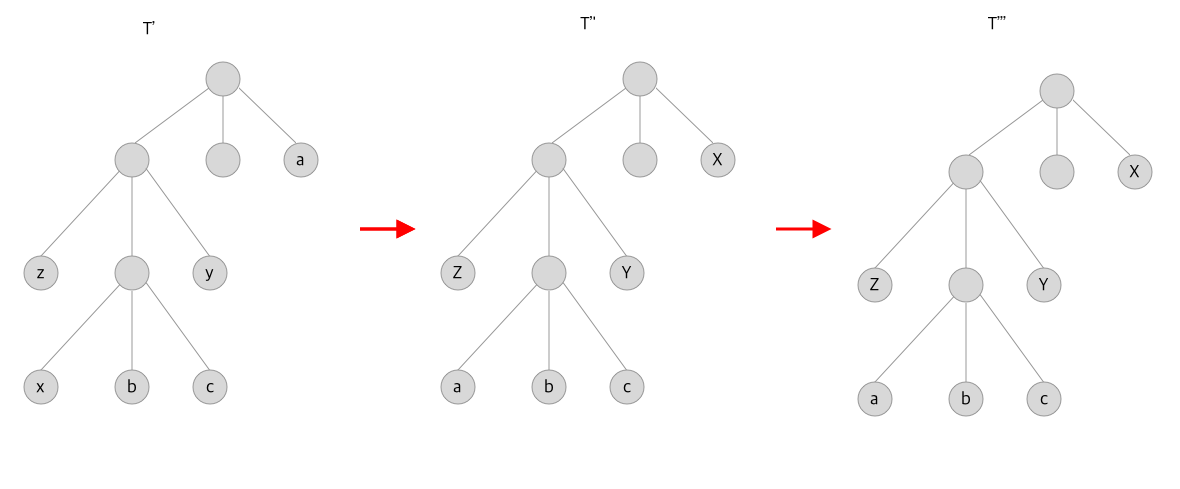
\includegraphics[width=\linewidth]{images/worksheet_2_solution_21.png}
            \end{center}

            \begin{align}
            B(T) - B(T') &= \sum\limits_{c \in C} c.freq \cdot d_T(c) - \sum\limits_{c \in C} c.freq \cdot d_{T'}(c)\\
            &= x.freq \cdot d_T(x) + a.freq \cdot d_T(a) - x.freq \cdot d_{T'}(x) - a.freq \cdot d_{T'}(a)\\
            &= x.freq \cdot d_T(x) + a.freq \cdot d_T(a) _ x.freq \cdot d_T(a) - a.freq \cdot d_T(x)\\
            &= (a.freq - x.freq)(d_T(a) - d_T(x))\\
            &\geq 0
            \end{align}

            \bigskip

            because both $a.freq - x.freq$ and $d_T(a) - d_T(x)$ are nonnegative. More specifically,
            $a.freq - x.freq$ is non-negative because $x$ is a minimum-frequency leaf, and $d_T(a) - d_T(x)$
            is non-negative because $a$ is leaf of maximum depth in $T$. Similarly, exchanging
            $y$ and $b$ does not increase the cost, and so $B(T') - B(T'')$ is non-negative.
            Therefore $B(T'') \leq B(T)$, and since $T$ is optimal we have $B(T) \leq B(T'')$,
            which implies $B(T) = B(T'')$. Thus $T''$ is an optimal tree in which $x$ and $y$
            appear as sibling leaves of maximum depth, from which the lemma follows.

            \end{proof}


            \item Proof of optimal structure property for Huffman's Algorithm (Ternary)

            \bigskip

            \underline{\textbf{Lemma (Modification of lemma on page 435):}}

            \bigskip

            Let $C$ be a given alphabet with frequency $c.freq$ defined for each
            character $c \in C$. Let $x$, $y$ and $z$ be three characters in $C$ with minimum frequency.
            Let $C'$ be the alphabet $C$ with characters $x$, $y$ and $z$ removed and a new character
            $w$ added, so that $C' = C - \{x,y,z\} \cup \{w\}$. Define $freq$ for $C'$ as for $C$, except taht
            $w.freq = x.freq + y.freq + z.freq$. Let $T'$ be any tree representing an optimal prefix code
            for the alphabet $C'$. Then the tree $T$, obtained from $T'$ by replacing the leaf node
            for $w$ with an internal node having $x$, $y$ and $z$ as children, represents an optimal prefix
            code for the alphabet $C$.

            \bigskip

            \begin{proof}
            We first show how to express the cost $B(T)$ of tree $T$ in terms of the cost
            $B(T')$ of the Tree $T'$ by considering the componentin equation 16.4.
            For each character $c \in C - \{x,y,z\}$, we have that $d_T(c) = d_{T'}(c)$, and hence
            $c.freq \cdot d_T(c) = c.freq \cdot d_{T'}(c)$. Since $d_T(w) = d_T(x) = d_T(y) = d_{T'}(z) + 1$, we have
            $w.freq = x.freq + y.freq + z.freq$.
            \end{proof}


        \end{itemize}


    \end{mdframed}
    \bigskip

    \underline{\textbf{Notes:}}

    \bigskip

    \begin{itemize}
        \item Lemma means ``subsidiary or intermediate theorem in an argument of proof''
        \item Proof of greedy-choice property for Huffman's Algorithm (Binary)

        \bigskip

        \underline{\textbf{Lemma 16.2:}}

        \bigskip

        Let $C$ be an alphabet in which each chapter $c \in C$ has frequency $c.freq$. Let
        $x$ and $y$ be two characters in $C$ having the lowest frequencies. Then there exists an
        optimal prefix code for $C$ in which the codewords for $x$ and $y$ have the same
        length and differ only in the last bit.

        \bigskip

        \begin{proof}

        \end{proof}
        \item Proof of optimal structure property for Huffman's Algorithm (Binary)

        \bigskip
    \end{itemize}

\end{enumerate}

\end{document}